\chapter{Figures}
\section{Séries temporelles}
\begin{figure}[h]
	\centering
    \begin{subfigure}[b]{\textwidth}
    	\centering
     	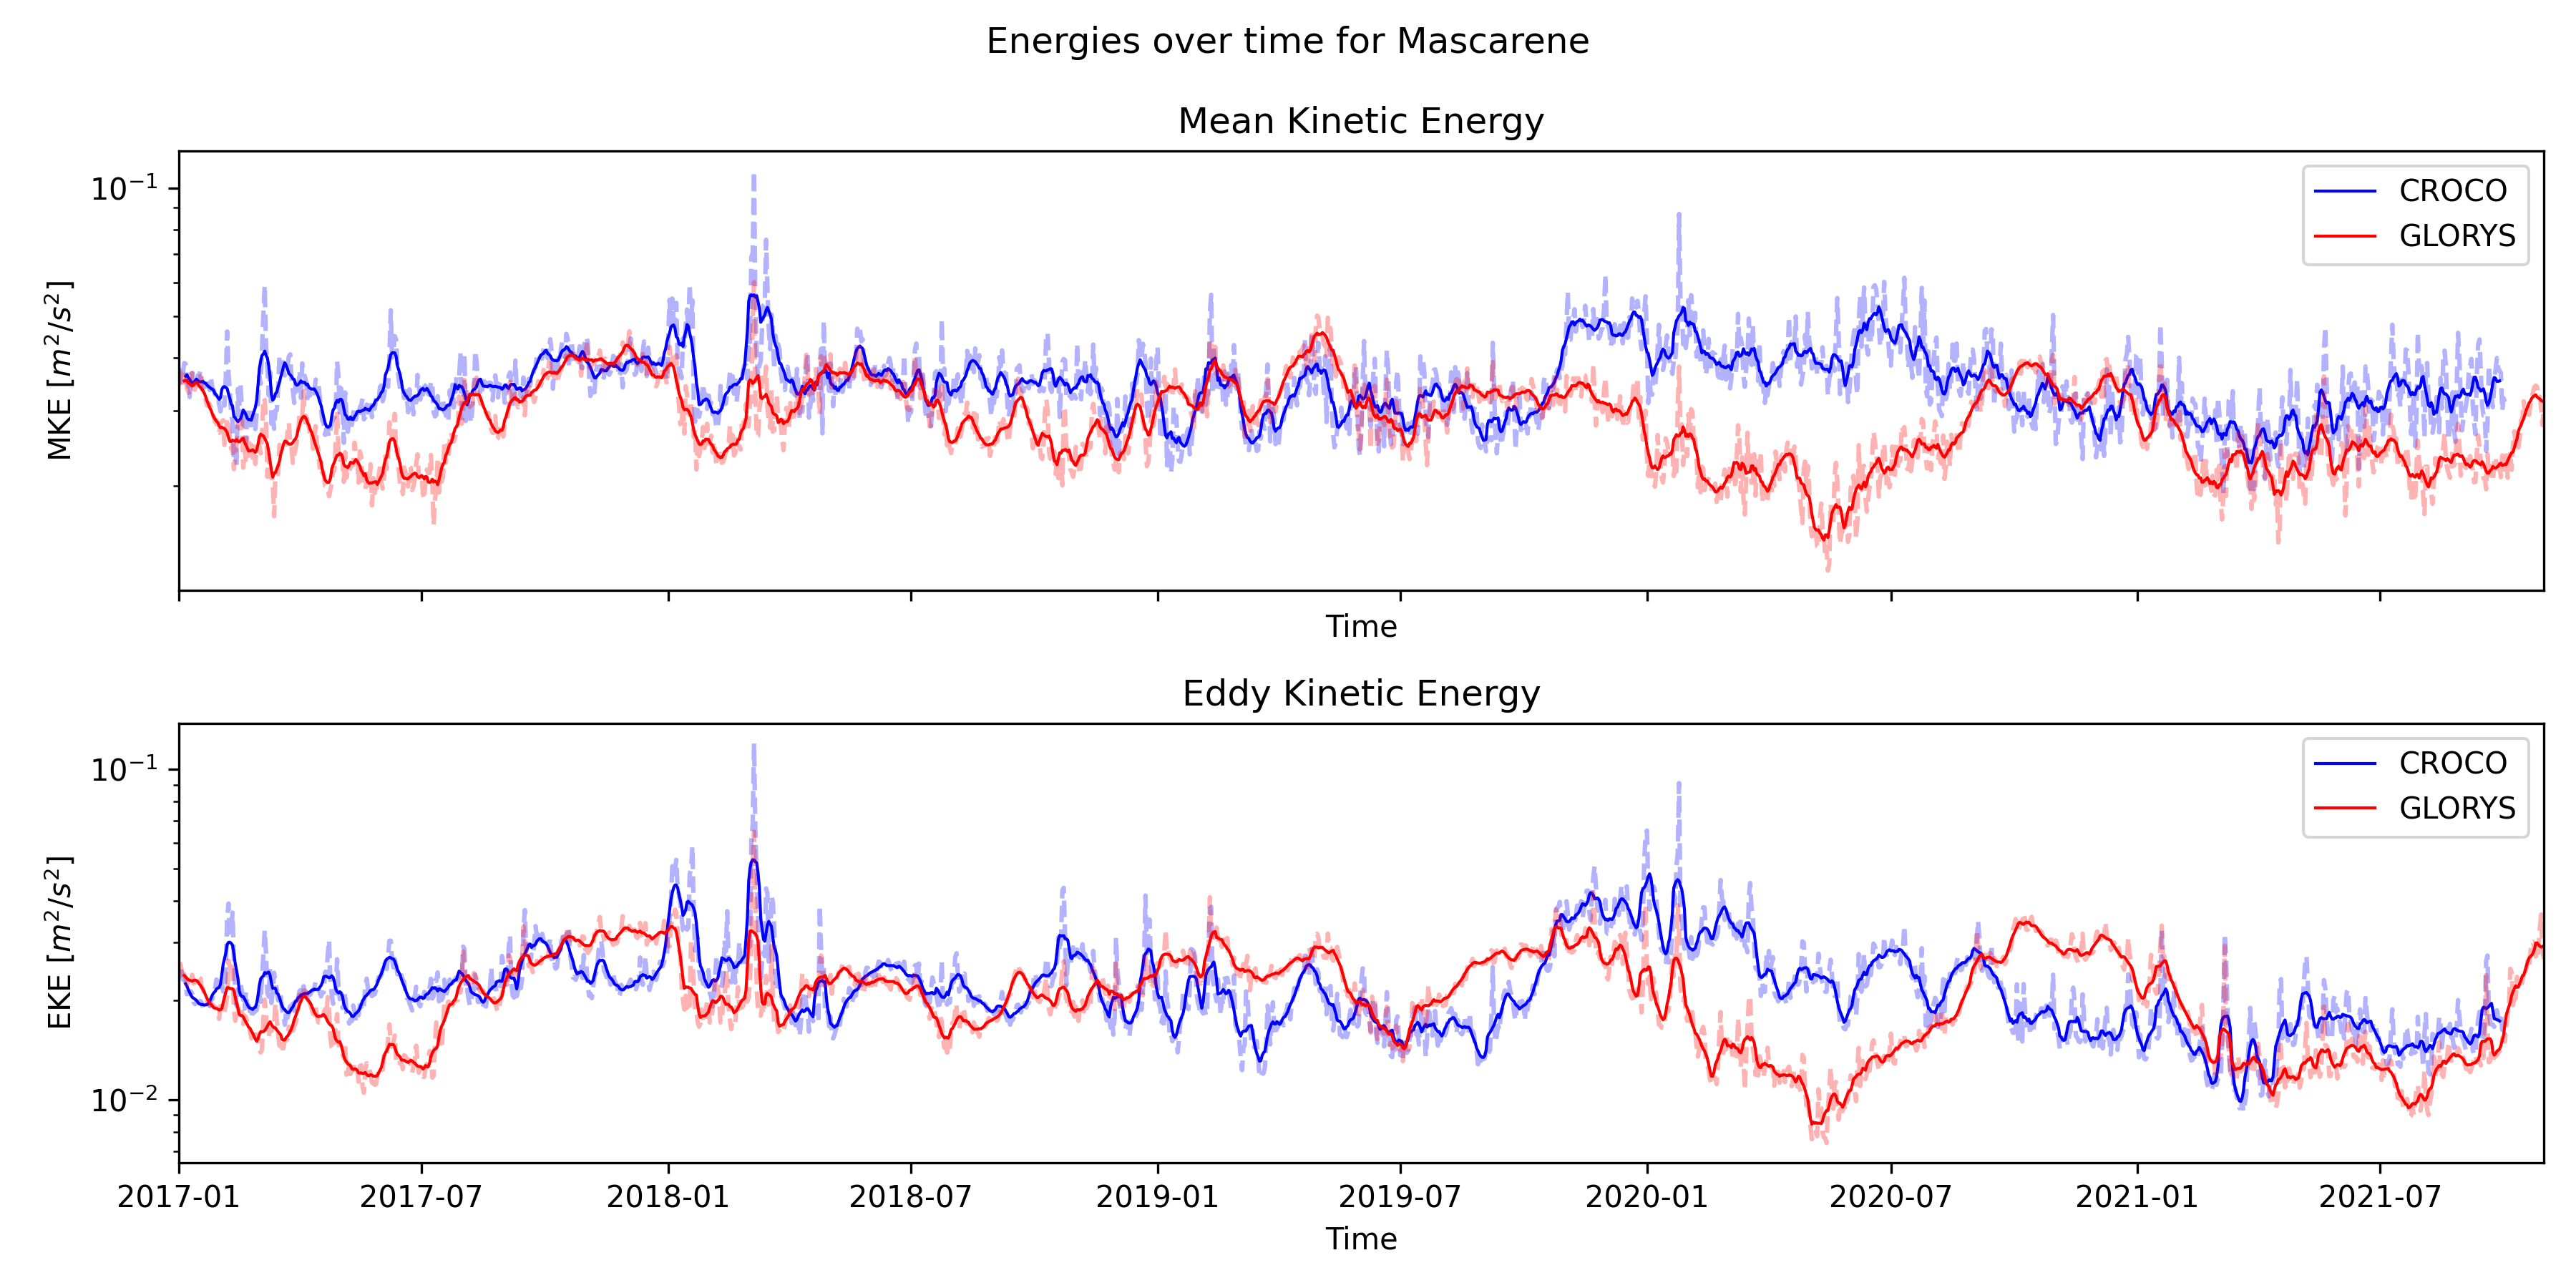
\includegraphics[width=0.9\textwidth]{Figures/Mascarene_energies_time_series}
     	\caption{Séries temporelles pour la région des îles Mascarene}
    \end{subfigure}
	\begin{subfigure}[b]{\textwidth}
		\centering
		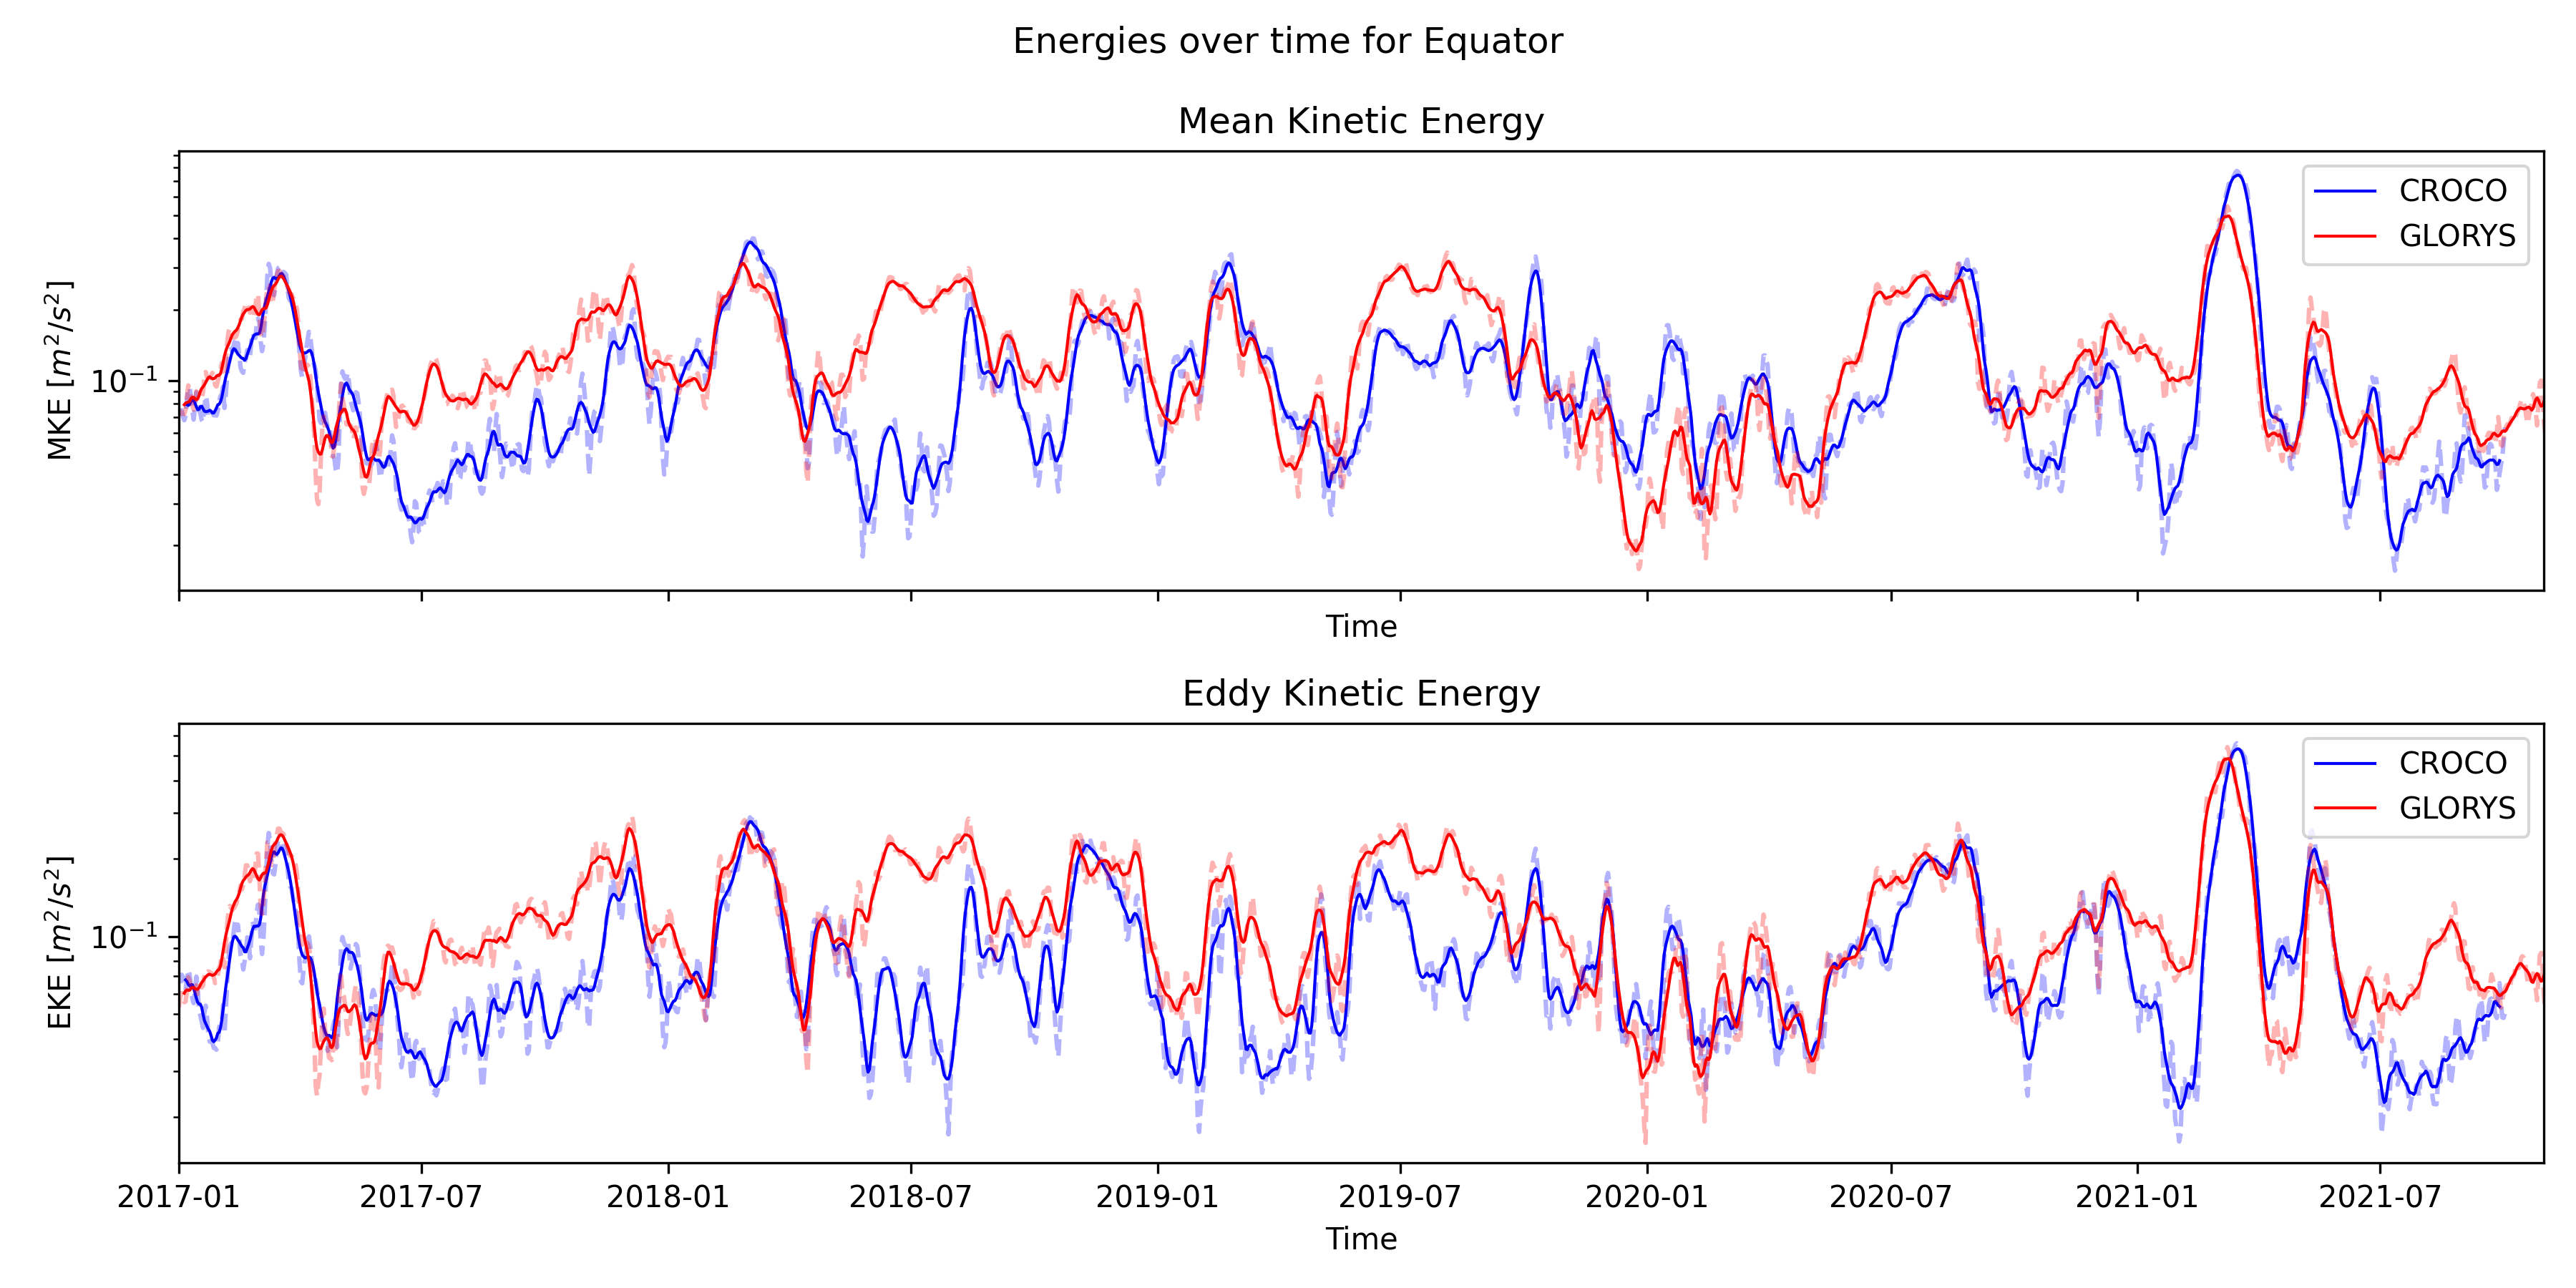
\includegraphics[width=0.9\textwidth]{Figures/Equator_energies_time_series}
		\caption{Séries temporelles pour la région de l'Équateur}
	\end{subfigure}
    \caption{Séries temporelles des énergies}
    \label{fig:ST Energy deter 2}
\end{figure}

\begin{figure}[h]
	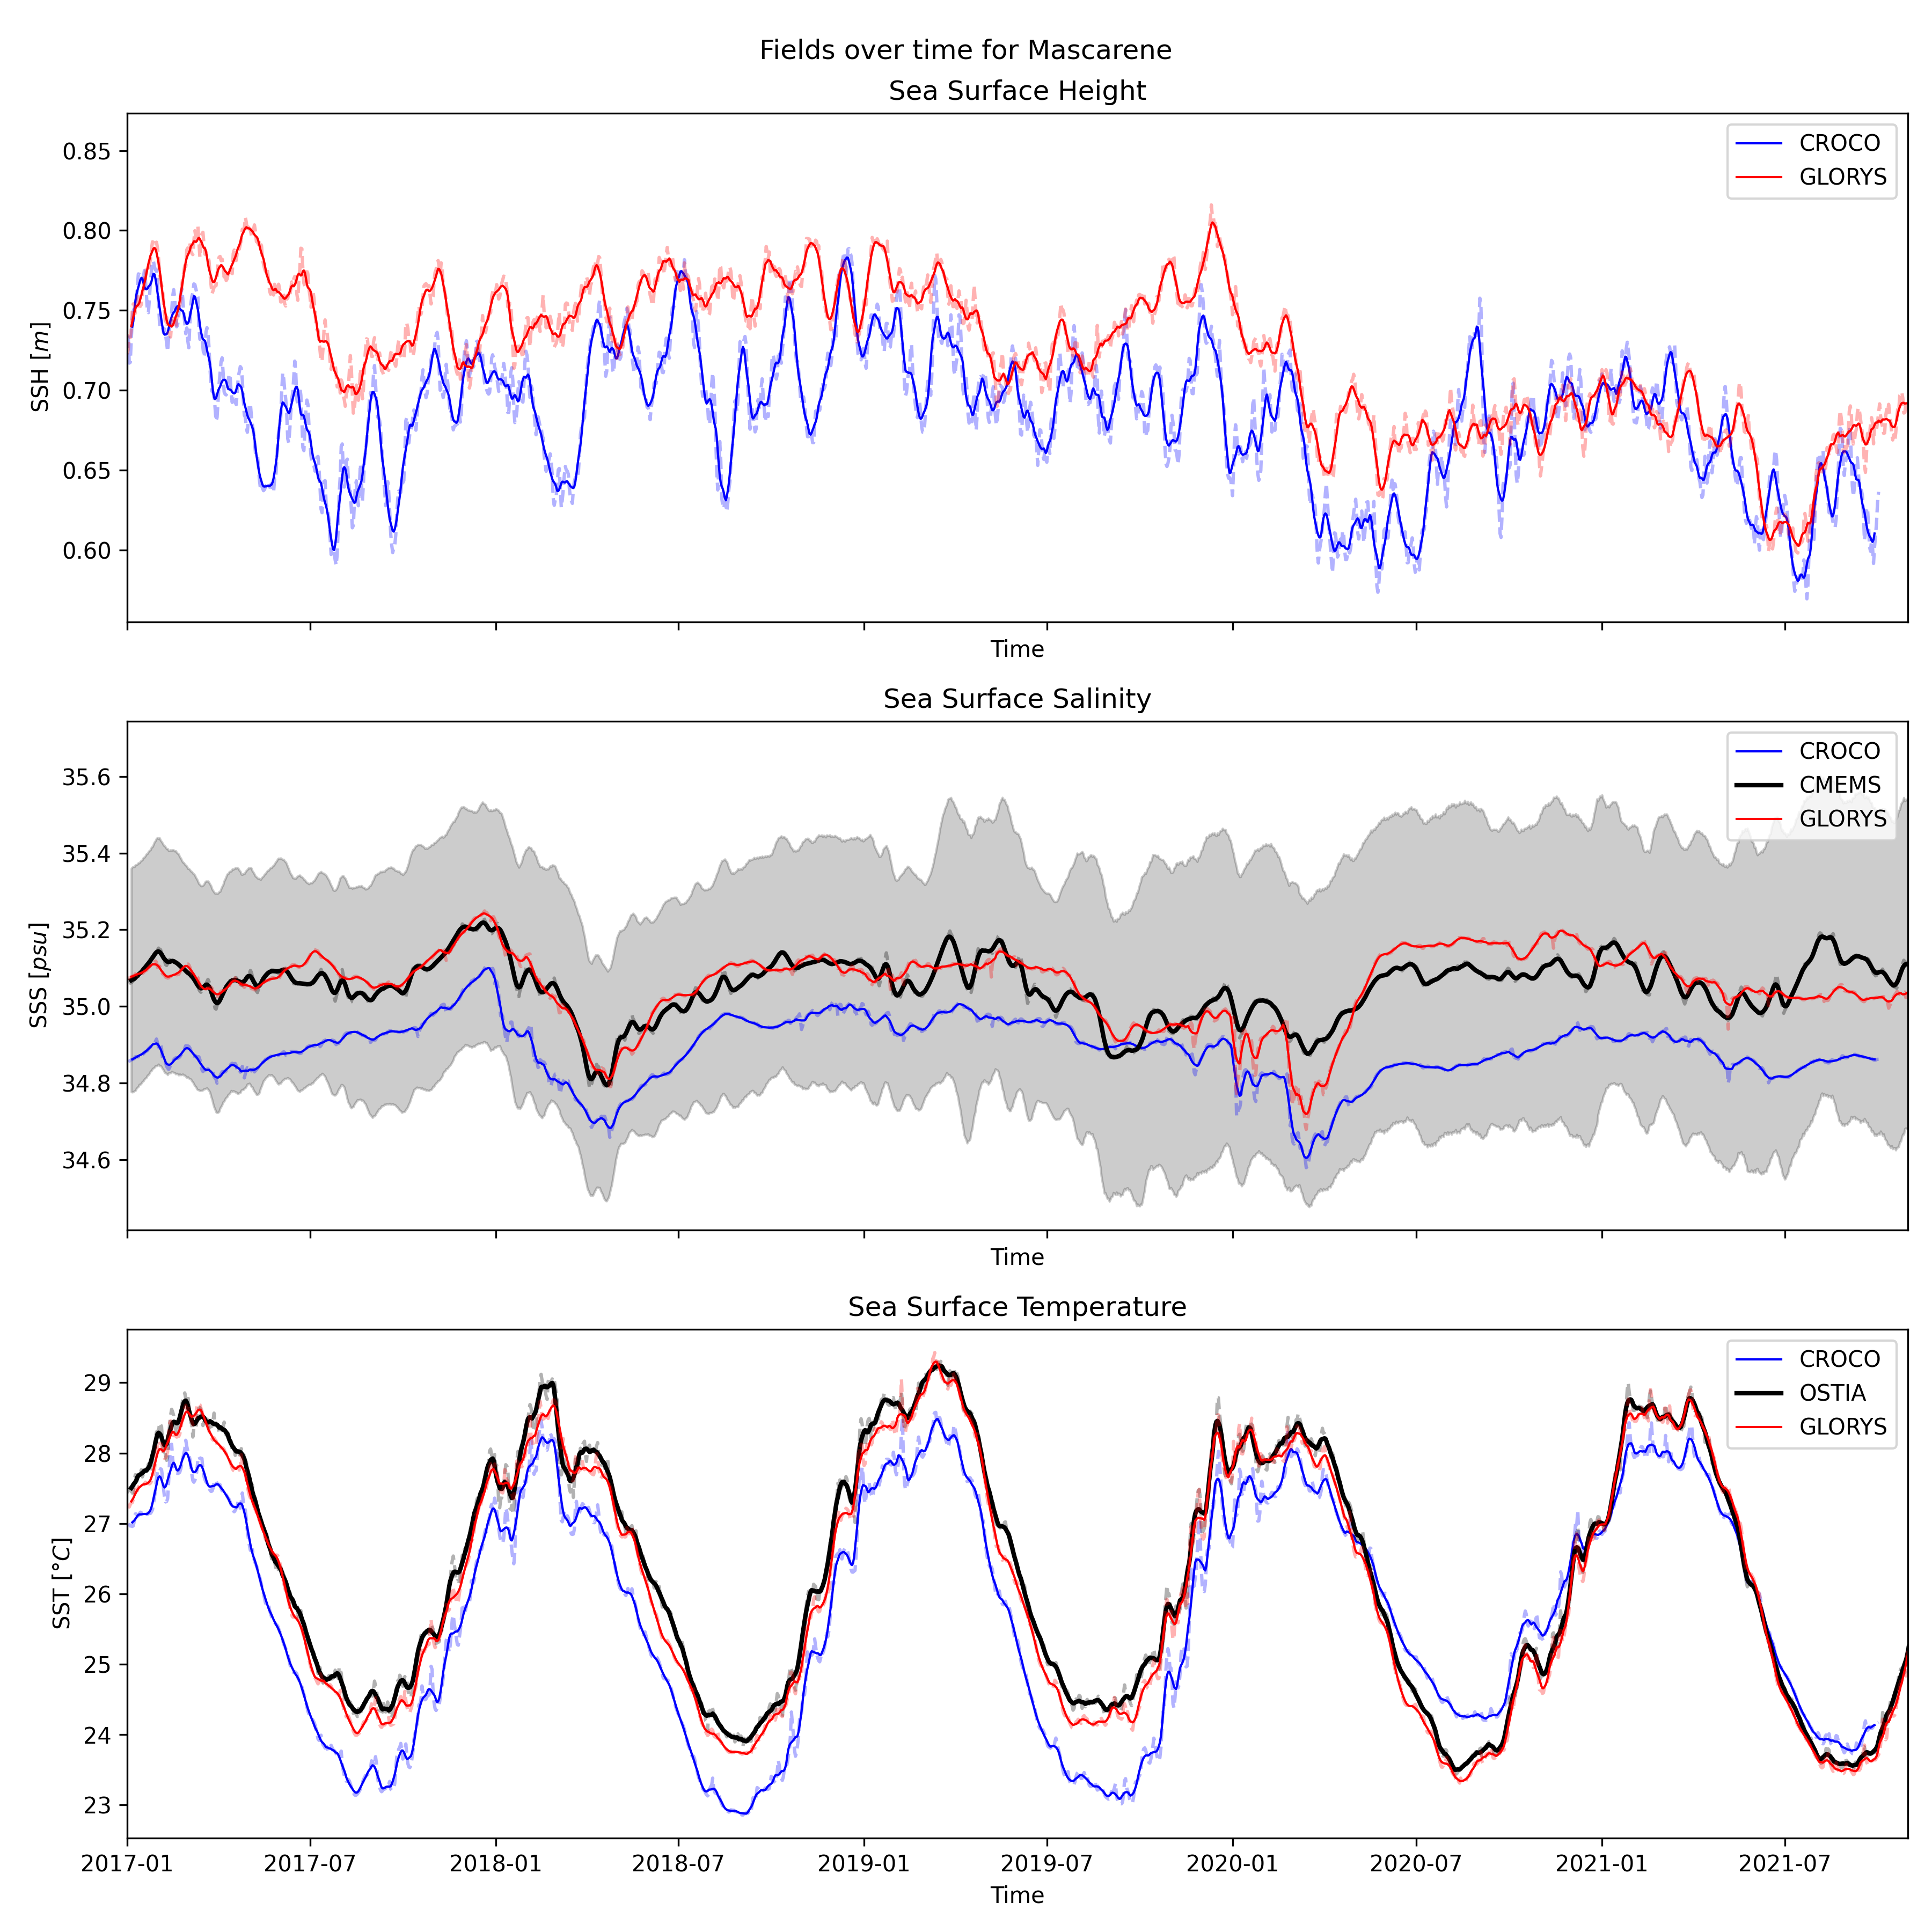
\includegraphics[width=\textwidth]{Figures/Mascarene_fields_time_series}
	\caption{Séries temporelles des traceurs de surface pour la région des îles Mascarene}
	\label{fig:ST Mascarene deter}
\end{figure}

\begin{figure}[h]
	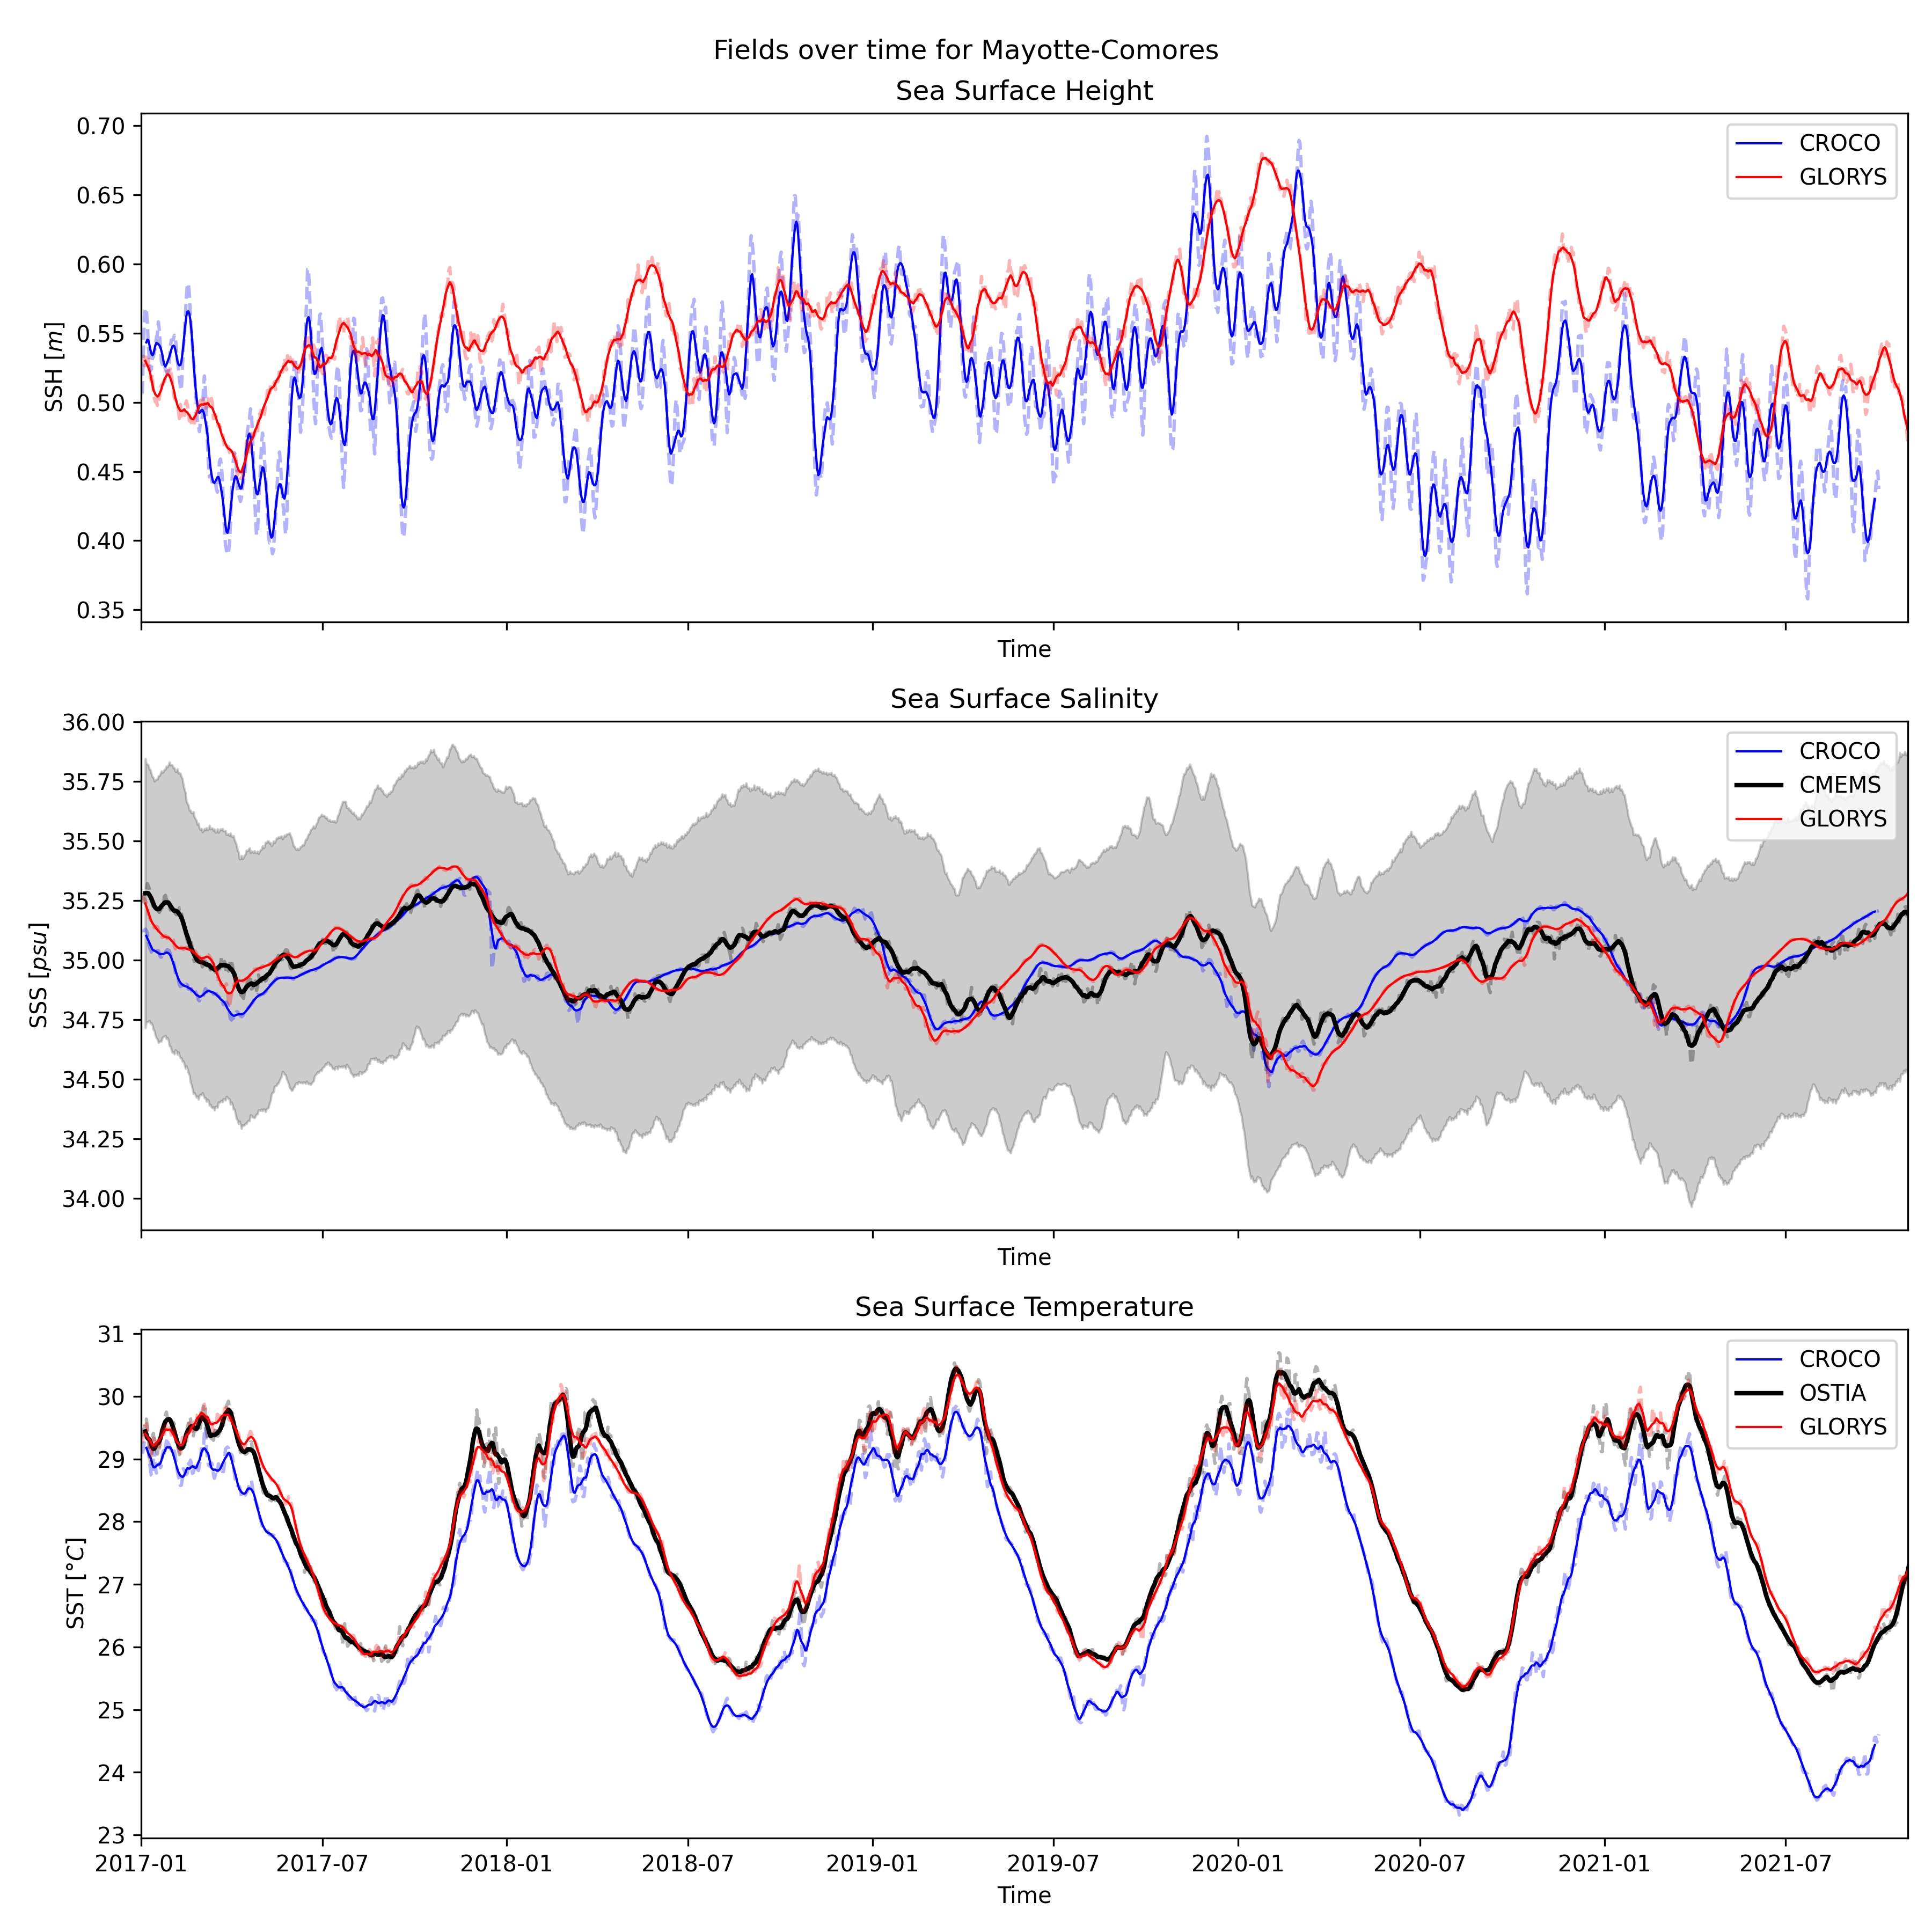
\includegraphics[width=\textwidth]{Figures/Mayotte-Comores_fields_time_series}
	\caption{Séries temporelles des traceurs de surface pour la région de Mayotte et des Comores}
	\label{fig:ST Mayotte deter}
\end{figure}

\begin{figure}[h]
	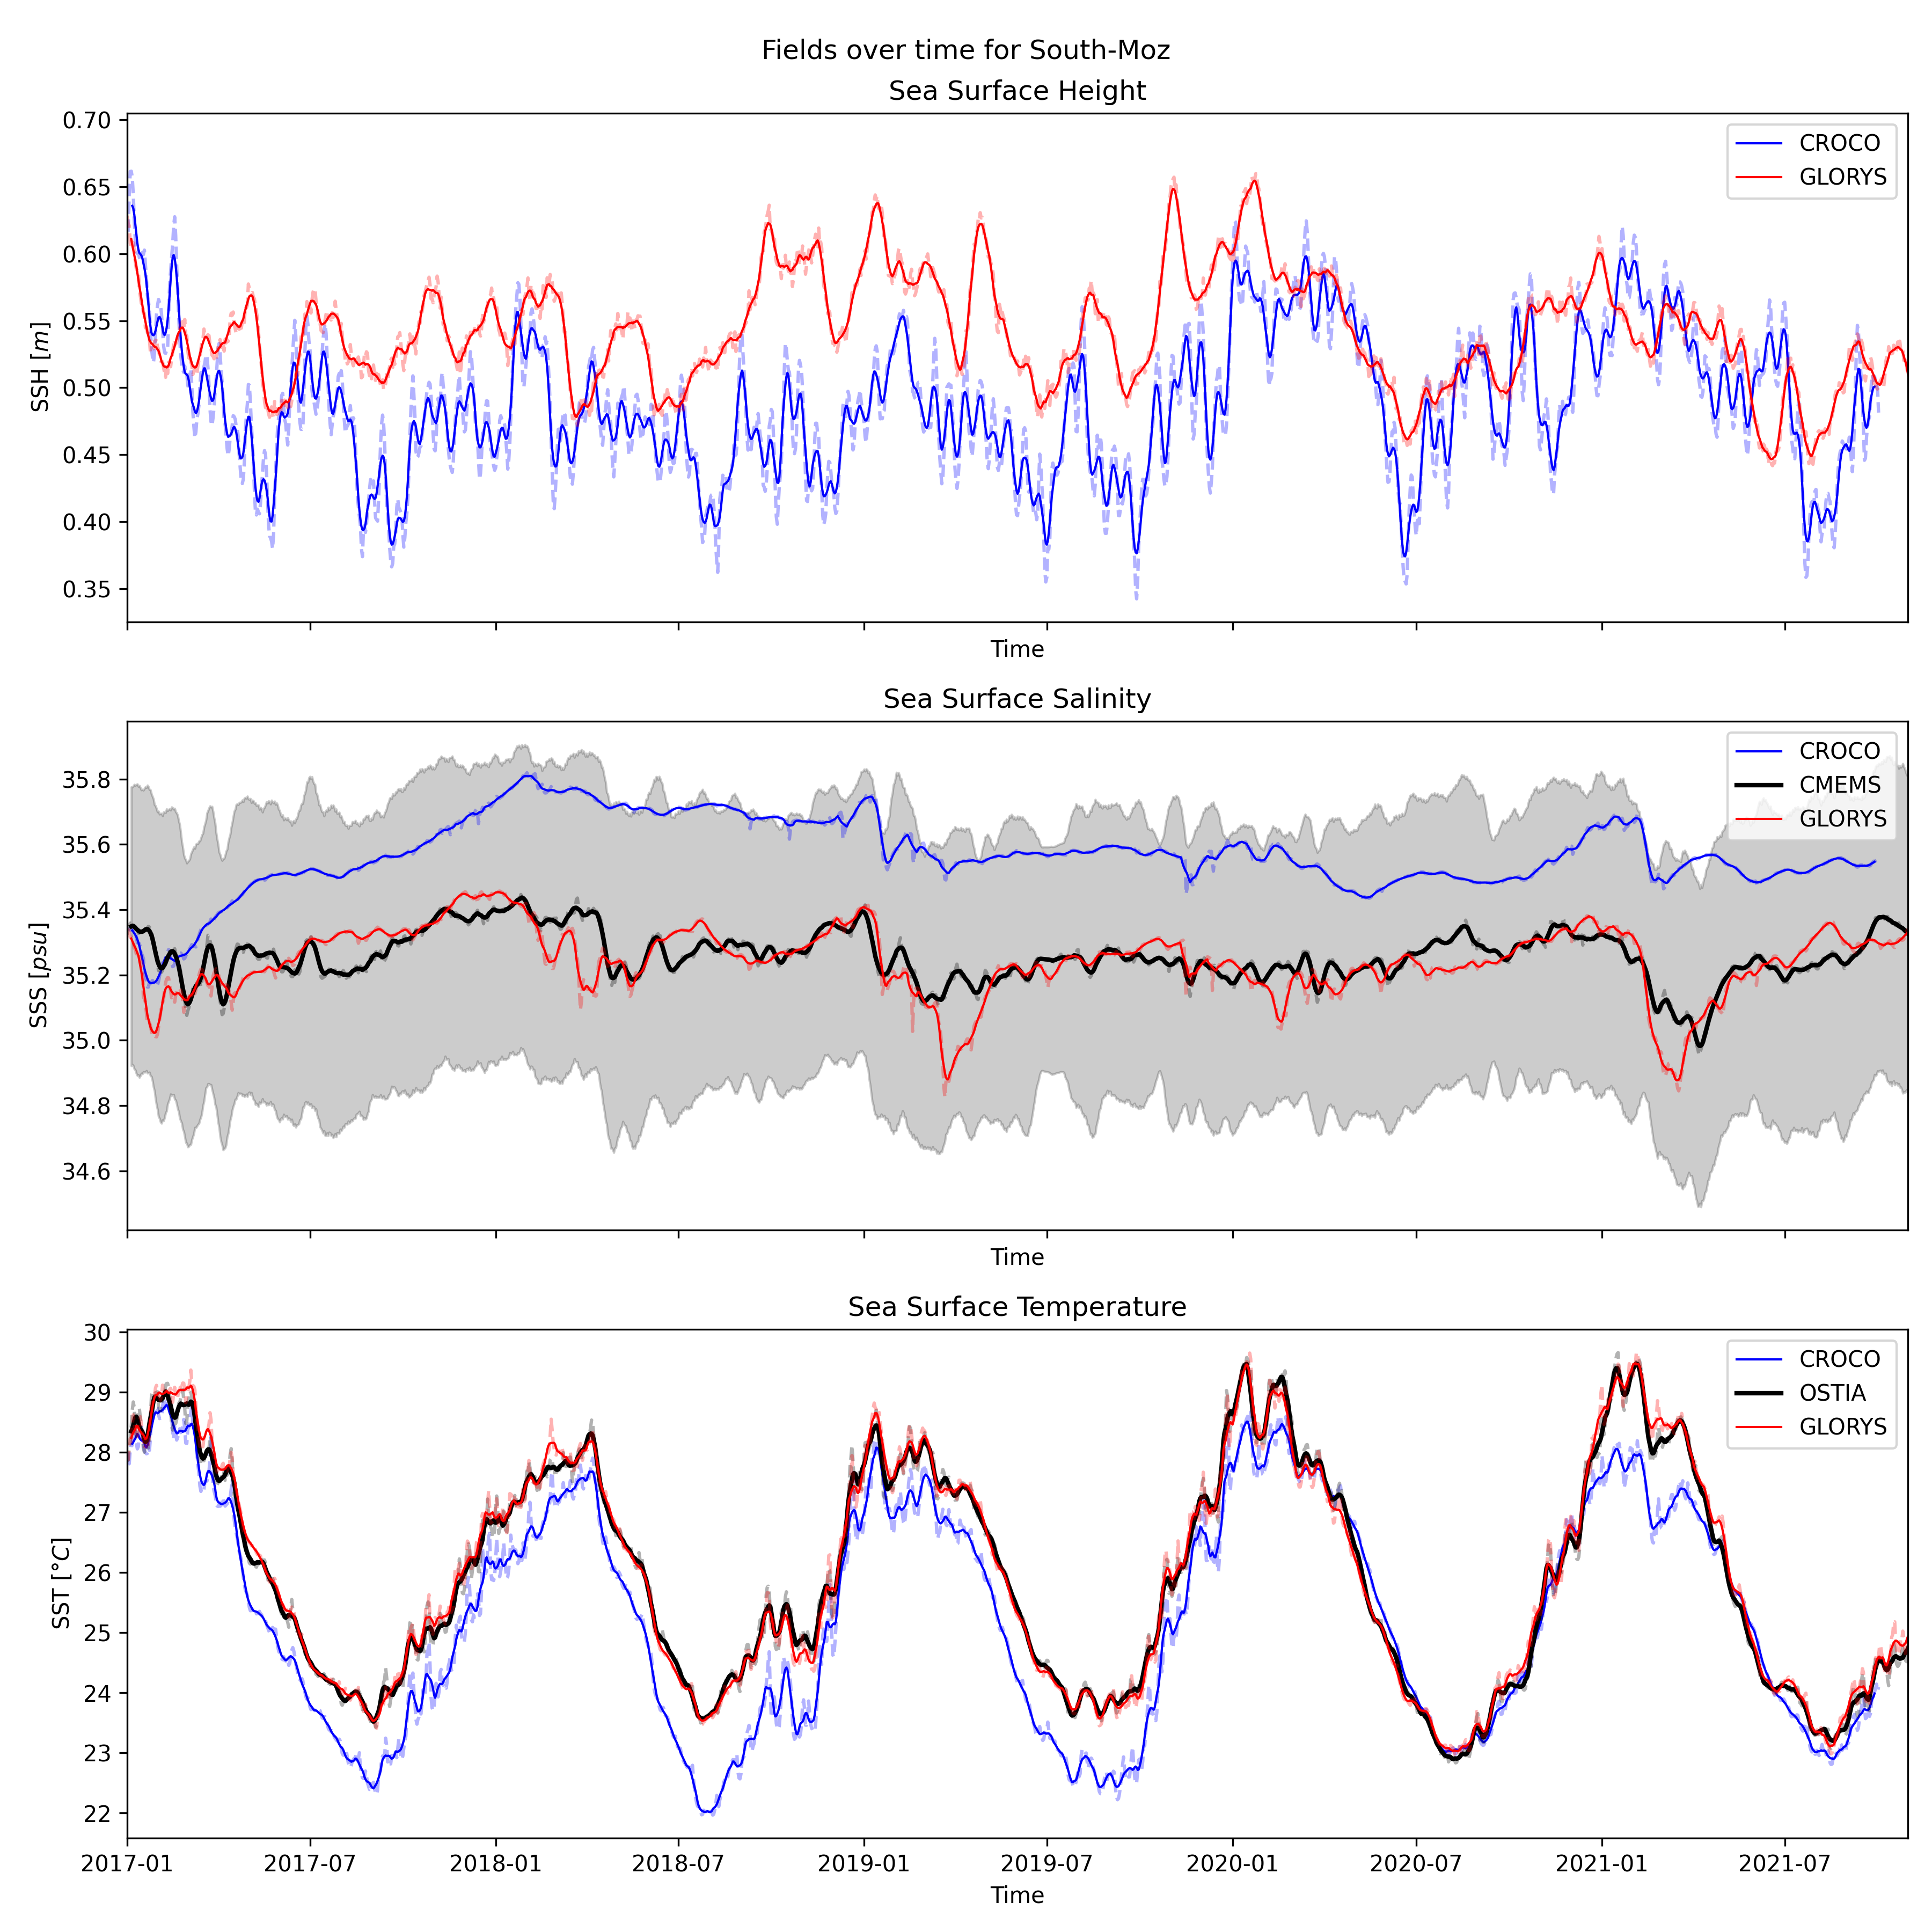
\includegraphics[width=\textwidth]{Figures/South-Moz_fields_time_series}
	\caption{Séries temporelles des traceurs de surface pour la région du sud du canal du Mozambique}
	\label{fig:ST South Moz deter}
\end{figure}